% Options for packages loaded elsewhere
\PassOptionsToPackage{unicode}{hyperref}
\PassOptionsToPackage{hyphens}{url}
\PassOptionsToPackage{dvipsnames,svgnames,x11names}{xcolor}
%
\documentclass[
  letterpaper,
  DIV=11,
  numbers=noendperiod]{scrreport}

\usepackage{amsmath,amssymb}
\usepackage{iftex}
\ifPDFTeX
  \usepackage[T1]{fontenc}
  \usepackage[utf8]{inputenc}
  \usepackage{textcomp} % provide euro and other symbols
\else % if luatex or xetex
  \usepackage{unicode-math}
  \defaultfontfeatures{Scale=MatchLowercase}
  \defaultfontfeatures[\rmfamily]{Ligatures=TeX,Scale=1}
\fi
\usepackage{lmodern}
\ifPDFTeX\else  
    % xetex/luatex font selection
\fi
% Use upquote if available, for straight quotes in verbatim environments
\IfFileExists{upquote.sty}{\usepackage{upquote}}{}
\IfFileExists{microtype.sty}{% use microtype if available
  \usepackage[]{microtype}
  \UseMicrotypeSet[protrusion]{basicmath} % disable protrusion for tt fonts
}{}
\makeatletter
\@ifundefined{KOMAClassName}{% if non-KOMA class
  \IfFileExists{parskip.sty}{%
    \usepackage{parskip}
  }{% else
    \setlength{\parindent}{0pt}
    \setlength{\parskip}{6pt plus 2pt minus 1pt}}
}{% if KOMA class
  \KOMAoptions{parskip=half}}
\makeatother
\usepackage{xcolor}
\setlength{\emergencystretch}{3em} % prevent overfull lines
\setcounter{secnumdepth}{5}
% Make \paragraph and \subparagraph free-standing
\makeatletter
\ifx\paragraph\undefined\else
  \let\oldparagraph\paragraph
  \renewcommand{\paragraph}{
    \@ifstar
      \xxxParagraphStar
      \xxxParagraphNoStar
  }
  \newcommand{\xxxParagraphStar}[1]{\oldparagraph*{#1}\mbox{}}
  \newcommand{\xxxParagraphNoStar}[1]{\oldparagraph{#1}\mbox{}}
\fi
\ifx\subparagraph\undefined\else
  \let\oldsubparagraph\subparagraph
  \renewcommand{\subparagraph}{
    \@ifstar
      \xxxSubParagraphStar
      \xxxSubParagraphNoStar
  }
  \newcommand{\xxxSubParagraphStar}[1]{\oldsubparagraph*{#1}\mbox{}}
  \newcommand{\xxxSubParagraphNoStar}[1]{\oldsubparagraph{#1}\mbox{}}
\fi
\makeatother


\providecommand{\tightlist}{%
  \setlength{\itemsep}{0pt}\setlength{\parskip}{0pt}}\usepackage{longtable,booktabs,array}
\usepackage{calc} % for calculating minipage widths
% Correct order of tables after \paragraph or \subparagraph
\usepackage{etoolbox}
\makeatletter
\patchcmd\longtable{\par}{\if@noskipsec\mbox{}\fi\par}{}{}
\makeatother
% Allow footnotes in longtable head/foot
\IfFileExists{footnotehyper.sty}{\usepackage{footnotehyper}}{\usepackage{footnote}}
\makesavenoteenv{longtable}
\usepackage{graphicx}
\makeatletter
\def\maxwidth{\ifdim\Gin@nat@width>\linewidth\linewidth\else\Gin@nat@width\fi}
\def\maxheight{\ifdim\Gin@nat@height>\textheight\textheight\else\Gin@nat@height\fi}
\makeatother
% Scale images if necessary, so that they will not overflow the page
% margins by default, and it is still possible to overwrite the defaults
% using explicit options in \includegraphics[width, height, ...]{}
\setkeys{Gin}{width=\maxwidth,height=\maxheight,keepaspectratio}
% Set default figure placement to htbp
\makeatletter
\def\fps@figure{htbp}
\makeatother
% definitions for citeproc citations
\NewDocumentCommand\citeproctext{}{}
\NewDocumentCommand\citeproc{mm}{%
  \begingroup\def\citeproctext{#2}\cite{#1}\endgroup}
\makeatletter
 % allow citations to break across lines
 \let\@cite@ofmt\@firstofone
 % avoid brackets around text for \cite:
 \def\@biblabel#1{}
 \def\@cite#1#2{{#1\if@tempswa , #2\fi}}
\makeatother
\newlength{\cslhangindent}
\setlength{\cslhangindent}{1.5em}
\newlength{\csllabelwidth}
\setlength{\csllabelwidth}{3em}
\newenvironment{CSLReferences}[2] % #1 hanging-indent, #2 entry-spacing
 {\begin{list}{}{%
  \setlength{\itemindent}{0pt}
  \setlength{\leftmargin}{0pt}
  \setlength{\parsep}{0pt}
  % turn on hanging indent if param 1 is 1
  \ifodd #1
   \setlength{\leftmargin}{\cslhangindent}
   \setlength{\itemindent}{-1\cslhangindent}
  \fi
  % set entry spacing
  \setlength{\itemsep}{#2\baselineskip}}}
 {\end{list}}
\usepackage{calc}
\newcommand{\CSLBlock}[1]{\hfill\break\parbox[t]{\linewidth}{\strut\ignorespaces#1\strut}}
\newcommand{\CSLLeftMargin}[1]{\parbox[t]{\csllabelwidth}{\strut#1\strut}}
\newcommand{\CSLRightInline}[1]{\parbox[t]{\linewidth - \csllabelwidth}{\strut#1\strut}}
\newcommand{\CSLIndent}[1]{\hspace{\cslhangindent}#1}

\KOMAoption{captions}{tableheading}
\makeatletter
\@ifpackageloaded{bookmark}{}{\usepackage{bookmark}}
\makeatother
\makeatletter
\@ifpackageloaded{caption}{}{\usepackage{caption}}
\AtBeginDocument{%
\ifdefined\contentsname
  \renewcommand*\contentsname{Tabla de contenidos}
\else
  \newcommand\contentsname{Tabla de contenidos}
\fi
\ifdefined\listfigurename
  \renewcommand*\listfigurename{Listado de Figuras}
\else
  \newcommand\listfigurename{Listado de Figuras}
\fi
\ifdefined\listtablename
  \renewcommand*\listtablename{Listado de Tablas}
\else
  \newcommand\listtablename{Listado de Tablas}
\fi
\ifdefined\figurename
  \renewcommand*\figurename{Figura}
\else
  \newcommand\figurename{Figura}
\fi
\ifdefined\tablename
  \renewcommand*\tablename{Tabla}
\else
  \newcommand\tablename{Tabla}
\fi
}
\@ifpackageloaded{float}{}{\usepackage{float}}
\floatstyle{ruled}
\@ifundefined{c@chapter}{\newfloat{codelisting}{h}{lop}}{\newfloat{codelisting}{h}{lop}[chapter]}
\floatname{codelisting}{Listado}
\newcommand*\listoflistings{\listof{codelisting}{Listado de Listados}}
\makeatother
\makeatletter
\makeatother
\makeatletter
\@ifpackageloaded{caption}{}{\usepackage{caption}}
\@ifpackageloaded{subcaption}{}{\usepackage{subcaption}}
\makeatother

\ifLuaTeX
\usepackage[bidi=basic]{babel}
\else
\usepackage[bidi=default]{babel}
\fi
\babelprovide[main,import]{spanish}
% get rid of language-specific shorthands (see #6817):
\let\LanguageShortHands\languageshorthands
\def\languageshorthands#1{}
\ifLuaTeX
  \usepackage{selnolig}  % disable illegal ligatures
\fi
\usepackage{bookmark}

\IfFileExists{xurl.sty}{\usepackage{xurl}}{} % add URL line breaks if available
\urlstyle{same} % disable monospaced font for URLs
\hypersetup{
  pdftitle={Reloj inteligente IoT basado en tecnologías abiertas para la recopilación de datos de confort térmico},
  pdfauthor={Julio César Landa López},
  pdflang={es},
  colorlinks=true,
  linkcolor={blue},
  filecolor={Maroon},
  citecolor={Blue},
  urlcolor={Blue},
  pdfcreator={LaTeX via pandoc}}


\title{Reloj inteligente IoT basado en tecnologías abiertas para la
recopilación de datos de confort térmico}
\author{Julio César Landa López}
\date{2024-10-10}

\begin{document}
\maketitle

\renewcommand*\contentsname{Tabla de contenidos}
{
\hypersetup{linkcolor=}
\setcounter{tocdepth}{2}
\tableofcontents
}
\listoffigures
\listoftables

\bookmarksetup{startatroot}

\chapter*{Resumen}\label{resumen}
\addcontentsline{toc}{chapter}{Resumen}

\markboth{Resumen}{Resumen}

\bookmarksetup{startatroot}

\chapter*{Abstract}\label{abstract}
\addcontentsline{toc}{chapter}{Abstract}

\markboth{Abstract}{Abstract}

\bookmarksetup{startatroot}

\chapter*{Agradecimientos}\label{agradecimientos}
\addcontentsline{toc}{chapter}{Agradecimientos}

\markboth{Agradecimientos}{Agradecimientos}

Poner atención en el titulo, no convence ``Medición de confort
térmico'', no se puede medir el confort térmico

\bookmarksetup{startatroot}

\chapter{Introducción}\label{introducciuxf3n}

El reporte de Cambio Climático 2023 del Panel Intergubernamental sobre
Cambio Climático (IPCC) advierte sobre un probable aumento en la
temperatura superior a 1.5°C entre los años 2021 y 2040, alcanzando
hasta los 5.7°C para 2100 (Synthesis Report 2023). Para limitar este
calentamiento, es imprescindible una reducción drástica de las emisiones
globales de gases de efecto invernadero (GEI). Estas emisiones deben
alcanzar su máximo antes del año 2025 y luego disminuir en un 43\% para
el año 2030, llegando a cero neto para el año 2050, conforme los
Objetivos de Desarrollo Sostenible de la Organización de las Naciones
Unidas (2015).

Las emisiones de GEI generadas por el uso de energía representan el
73.2\% a nivel global, y el uso de energía en edificaciones constituye
el 17.5\%, desglosado en un 6.6\% en edificaciones no residenciales y un
10.9\% en edificaciones residenciales (Ritchie 2020). En México, el
sector residencial, comercial y público representa el 17.16\% del
consumo final de energía, de los cuales el 34.29\% corresponden a
consumo eléctrico (Secretaría de Energía 2023). En materia de eficiencia
energética, el principal desafío que enfrentan los edificios no
residenciales en México es su uso intensivo de electricidad (Lorentzen y
McNeil 2020).

La eficiencia energética desempeña un papel crucial en la lucha contra
el cambio climático al optimizar el uso de recursos. Avanzar hacía la
eficiencia energética implica reducir las emisiones de gases de efecto
invernadero (GEI), lo cual favorece la descarbonización del sistema
energético. Las fuente de energías renovables pueden ser un aliado
valioso en el camino a la eficiencia energética.

Además, es importante destacar que una parte esencial en la búsqueda de
la eficiencia energética en edificaciones es la aplicación de
estrategias de diseño bioclimático. Estas consisten en el diseño de la
edificación de acuerdo al clima del lugar donde estará construida
(Olgyay et~al. 1963). Esto propicia tener espacios que satisfagan las
necesidades y expectativas de los ocupantes, proporcionando condiciones
de confort térmico para una mejor calidad de vida y productividad.

La digitalización energética tiene como objetivo contribuir a la
eficiencia energética y la fiabilidad del sistema energético en su
conjunto mediante el análisis de datos y la integración de tecnologías
digitales en la producción, almacenamiento, distribución y consumo de
energía. Esto implica el uso de tecnologías emergentes como la
inteligencia artificial (IA) o el internet de las cosas (IoT) (Olabi,
Abdelkarem, y Jouhara 2023). Esto favorece indirectamente a la
sustentabilidad al respaldar la eficiencia energética y fortalecer la
fiabilidad del sistema energético.

Si bien la digitalización energética es prometedora en este sentido para
la eficiencia energética y la descarbonización, también presenta
desafíos debido a que se espera un aumento en la demanda de energía a
nivel global (Mitigation of Climate Change 2022). Para poder llevar a
cabo un proceso de digitalización energética adecuado que permita lograr
los objetivos de descarbonización, se debe buscar una democracia
energética con tres perspectivas clave: soberanía popular, un gobierno
participativo y propiedad civil (Judson, Fitch-Roy, y Soutar 2022).

En la búsqueda de un futuro sustentable, la transición hacia fuentes de
energía renovables, tecnologías eficientes, edificaciones sustentables y
una democracia energética son de vital importancia; aunado a la
creciente necesidad de abordar la crisis climática, el consumo
energético de edificaciones requiere de acciones inmediatas.

El confort térmico se define como una condición mental que expresa la
satisfacción con el ambiente, y es un juicio cognitivo influenciado por
procesos físicos, fisiológicos y otros factores (American Society of
Heating, Refrigerating and Air-Conditioning Engineers, Inc. 2017).
Desempeña un papel esencial en el consumo de energía en edificaciones,
pues está intrínsecamente ligado a la forma en que diseñamos las
edificaciones. Una gran parte del consumo de energía en estas se ocupa
en mantener condiciones óptimas de iluminación, temperatura y humedad
del aire, buscando obtener espacios con condiciones adecuadas para que
los ocupantes se encuentren confort térmico, lumínico y acústico.

Para el confort térmico se toman en cuenta siete variables físicas, las
cuales están relacionadas a la transferencia de calor entre el ocupante
y su entorno, así como a los modelos de predicción de confort térmico.
Estas variables incluyen la temperatura, humedad relativa y velocidad
del aire, temperatura radiante, presión atmosférica, aislamiento térmico
de la ropa y nivel metabólico del ocupante (Enescu 2017). Asimismo,
existen variables fisiológicas altamente relacionadas con el confort
térmico que pueden servir como indicadores, tales como la temperatura de
la piel, la frecuencia cardíaca y la variabilidad de la frecuencia
cardíaca (Bogatu et~al. 2023).

Durante la fase de diseño de una edificación, el empleo de modelos
predictivos de confort térmico se convierte en una herramienta esencial
para desarrollar estrategias efectivas de diseño bioclimático. Además,
es crucial realizar encuestas de evaluación durante la ocupación para
determinar el nivel de confort térmico y evaluar la efectividad de las
estrategias implementadas durante la fase de diseño. Estas encuestas se
basan principalmente en cuestionarios destinados a recabar la opinión de
los ocupantes sobre su experiencia ambiental, mientras que las
mediciones experimentales de las variables físicas que inciden en el
entorno sirven como un respaldo fundamental (Aguirre 2021).

En este contexto, la transición hacia edificaciones sustentables no se
trata solo de reducir el consumo energético, sino de hacerlo de manera
eficiente sin comprometer el confort térmico, acústico y lumínico.

Existen diversos modelos que se utilizan para la predicción del confort
térmico en edificaciones. Estos modelos se clasifican comúnmente en dos
categorías: para edificaciones con sistemas de aire acondicionado y para
edificaciones sin este tipo de sistemas. Entre los modelos para
edificaciones con sistemas de aire acondicionado, el modelo más
utilizado es el conocido como método Fanger, este método se basa en las
variables físicas relacionadas al confort térmico mencionadas
previamente. Estas variables se utilizan en ecuaciones para calcular el
índice de sensación térmica (PMV por sus siglas en inglés) y el
porcentaje de personas insatisfechas (PPD por sus siglas en inglés)
(Fanger 1970). Mientras que para los sistemas sin aire acondicionado
existen algunos modelos como el PMV adaptativo o el PMV extendido
(American Society of Heating, Refrigerating and Air-Conditioning
Engineers, Inc. 2017), entre otros, los cuales, se explicaran más a
detalle en el siguiente capítulo.

Un problema es la precisión de los modelos existentes como el caso del
método Fanger (PMV-PPD), un estudio realizado por Cheung et~al. (2019)
donde se determina la precisión del modelo con la base de datos de
confort térmico global del ASHRAE, reporta que el PMV tiene una
precisión del 34\% respecto a la sensación térmica observada, mientras
que el PPD puede llegar a sobrestimar la insatisfacción de los
ocupantes. Esto da pie a continuar con la investigación y desarrollo de
más modelos, como el caso de la implementación de algoritmos de
aprendizaje automático.

En años recientes se han utilizado nuevas herramientas como el caso de
los dispositivos wearables para el desarrollo de modelos de confort, la
implementación de dichos dispositivos con sensores integrados, tienen la
capacidad de medir variables ambientales y fisiológicas que permiten
generar bases de datos que incluyan datos fisiológicos de los ocupantes
y la obtención de modelos de confort más precisos.

En esta tesis se presenta el desarrollo de un prototipo de wearable con
software y hardware libres que recopile y envíe datos sobre encuestas de
confort térmico e información extra de variables fisiológicas a una
plataforma de IoT, con el fin de crear una base de datos que permita el
desarrollo de modelos de confort térmico. A continuación se presenta las
contribuciones de este proyecto.

\textbf{Medición precisa y en tiempo real de variables fisiológicas:} El
uso de un dispositivo wearable permite la captura directa de variables
fisiológicas relacionadas al confort térmico, como la temperatura
corporal y la frecuencia cardíaca.

\textbf{Monitoreo continuo y no intrusivo}: Al ser un dispositivo
portable y de uso constante, este permite el monitoreo continuo y no
intrusivo de las variables fisiológicas mencionadas previamente,
facilitando la recopilación de datos a lo largo del tiempo, lo cual es
fundamental para el análisis de patrones y tendencias en el confort
térmico.

\textbf{Encuestas de confort térmico simplificadas:} La función de
encuestas periódicas de confort térmico es una de las partes más
importantes en el desarrollo del dispositivo para la creación de una
base de datos. Estas encuestas permiten al usuario evaluar su nivel de
confort térmico de manera rápida y sencilla.

\textbf{Contextualización de los datos de confort térmico:} Al
integrarse el dispositivo a la red de Internet de las Cosas del
Instituto de Energías Renovables junto con los demás dispositivos de
medición de variables físicas previamente instalados en el instituto,
permite contextualizar los datos de confort térmico del usuario en
relación con las condiciones ambientales del entorno.

\textbf{Potencial desarrollo de modelos de confort térmico:} El
desarrollo de este proyecto a un futuro puede tomar dos vertientes. Una
en donde se puedan generar modelos de confort personalizados para cada
individuo, favoreciendo a la digitalización energética y la
automatización de espacios. Y la otra vertiente para generar modelos
predictivos de confort térmico contextualizados para la comunidad del
instituto.

\bookmarksetup{startatroot}

\chapter{Marco teórico}\label{marco-teuxf3rico}

-- Aquí van todos los antecedentes de confort térmico, ya están en el
archivo estado.qmd --

\subparagraph{Sensores de temperatura}\label{sensores-de-temperatura}

Los sensores de temperatura se clasifican en dos tipos principales:
sensores de contacto y sensores sin contacto. Los sensores de contacto,
a su vez, se subdividen en tres categorías según su método de medición:

\textbf{\emph{Termopares}}:Utilizan el efecto Seebeck para generar una
voltaje por la unión de dos metales diferentes.

\textbf{\emph{Termistores}}: Son resistores sensibles a la temperatura,
cuya resistencia eléctrica varía en función de los cambios de
temperatura. Están fabricados con materiales cerámicos o poliméricos.
Existen dos tipos principales: los NTC (coeficiente de temperatura
negativo) y los PTC (coeficiente de temperatura positivo).

\textbf{\emph{Detectores de temperatura de resistencia (RTD)}}: Utilizan
metales puros, como el platino, para medir la temperatura a través de la
variación lineal y predecible de su resistencia eléctrica.

Por otro lado, los sensores sin contacto incluyen los sensores
infrarrojos, diseñados para detectar la radiación infrarroja emitida por
un objeto a distancia.

En el sector de la salud, los termistores son ampliamente utilizados
debido a su alta precisión en los rangos de temperatura corporal y su
rápida respuesta a los cambios de temperatura. Sin embargo, a raíz de la
pandemia de COVID-19 en 2020, el uso de sensores infrarrojos se
populariza considerablemente. Esto ha impulsado avances en su
tecnología, lo que los hace cada vez más comunes para medir la
temperatura corporal.

\bookmarksetup{startatroot}

\chapter{Desarrollo y construcción}\label{desarrollo-y-construcciuxf3n}

En esta sección se detalla el proceso de desarrollo y construcción del
dispositivo presentado en esta tesis. Se presenta una metodología en
donde se aborda una descripción general del dispositivo, la selección y
justificación de los componentes a utilizar. Se aborda la etapa de
diseño y construcción del dispositivo, el diseño e implementación de las
encuestas a través de la interfaz gráfica. Se describe también el
proceso de calibración de los sensores utilizados para garantizar
precisión y mediciones fiables. Finalmente, se detalla la conexión del
dispositivo a una plataforma IoT para el almacenamiento de los datos.

\section{Metodología}\label{metodologuxeda}

\begin{enumerate}
\def\labelenumi{\arabic{enumi}.}
\tightlist
\item
  \textbf{Descripción general del dispositivo:}
\end{enumerate}

El dispositivo presentado en esta tesis es un prototipo de reloj
inteligente diseñado específicamente para la investigación en el ámbito
del confort térmico. Este dispositivo permite la recopilación de datos
fisiológicos, tales como la frecuencia cardíaca y la temperatura de la
piel, variables cuya relación con el confort térmico se discutió en el
capítulo anterior. Además, este dispositivo realiza encuestas periódicas
simplificadas de confort térmico mediante una interfaz de usuario
intuitiva, que permite responder la encuesta de forma rápida y sencilla.
La recopilación de estos datos se realiza en la plataforma de IoT
llamada ThingsBoard, lo que permite la creación de una base de datos de
confort térmico en un bioclima cálido semihúmedo (Infonavit 2024) en
Temixco, Morelos. Esta base de datos facilitará estudios para el
entendimiento del confort térmico y el desarrollo de modelos de confort
para este tipo de bioclima, así como de modelos de confort
personalizados.

\begin{enumerate}
\def\labelenumi{\arabic{enumi}.}
\setcounter{enumi}{1}
\tightlist
\item
  \textbf{Selección de componentes}
\end{enumerate}

Para garantizar el funcionamiento preciso y adecuado del dispositivo, es
fundamental seleccionar correctamente todos los componentes. A
continuación se describen los principales componentes utilizados, junto
con sus características y la justificación de su elección en el
proyecto. Esta justificación se basa en criterios como compatibilidad,
consumo energético, precisión y capacidad de procesamiento en el caso
del microcontrolador.

Los componentes principales son los siguientes:

\begin{itemize}
\tightlist
\item
  Placa de desarrollo
\item
  Pantalla
\item
  Batería
\item
  Sensores
\end{itemize}

\textbf{Placa de desarrollo}

La selección de la tarjeta o placa de desarrollo es una decisión crucial
en el desarrollo del proyecto. Se requiere una placa de tamaño reducido
que cumpla con características esenciales como conexión WiFi, velocidad
de procesamiento, memoria y comunicación I2C. Además, debe tener un bajo
consumo energético para garantizar el uso portátil prolongado del
dispositivo.

Se buscan placas compactas con conectividad inalámbrica. Opciones con
microcontroladores como los de Arduino, ESP y Raspberry ofrecen estas
características.

Durante el proceso de selección se identifican dos placas con pantallas
integradas, que aunque podrían ser útiles, no cumplen con los requisitos
del proyecto. La placa LILYGO TTGO, no cuenta con tecnología táctil, lo
cual limita su utilidad para realizar encuestas de confort térmico. Por
otro lado, la MCU RP2040 con LCD redondo de 1.28 pulgadas, aunque cuenta
con una pantalla táctil, no ofrece conectividad WiFi, un requisito
esencial. Aunque estas dos placas no son tomadas en cuanta por las
razones ya mencionadas, sirven como referencia para la búsqueda de otras
opciones. En la tabla Tabla~\ref{tbl-placas} se presenta una comparación
de diferentes placas de desarrollo con las características requeridas.

\begin{longtable}[]{@{}
  >{\raggedright\arraybackslash}p{(\columnwidth - 10\tabcolsep) * \real{0.2778}}
  >{\raggedright\arraybackslash}p{(\columnwidth - 10\tabcolsep) * \real{0.0556}}
  >{\raggedright\arraybackslash}p{(\columnwidth - 10\tabcolsep) * \real{0.1019}}
  >{\raggedright\arraybackslash}p{(\columnwidth - 10\tabcolsep) * \real{0.3056}}
  >{\raggedright\arraybackslash}p{(\columnwidth - 10\tabcolsep) * \real{0.1204}}
  >{\raggedright\arraybackslash}p{(\columnwidth - 10\tabcolsep) * \real{0.1389}}@{}}
\caption{Comparación de características de conectividad y hardware en
placas de desarrollo}\label{tbl-placas}\tabularnewline
\toprule\noalign{}
\begin{minipage}[b]{\linewidth}\raggedright
Placa de desarrollo
\end{minipage} & \begin{minipage}[b]{\linewidth}\raggedright
Wifi
\end{minipage} & \begin{minipage}[b]{\linewidth}\raggedright
Bluetooth
\end{minipage} & \begin{minipage}[b]{\linewidth}\raggedright
Comunicación
\end{minipage} & \begin{minipage}[b]{\linewidth}\raggedright
Cable
\end{minipage} & \begin{minipage}[b]{\linewidth}\raggedright
Pines
\end{minipage} \\
\midrule\noalign{}
\endfirsthead
\toprule\noalign{}
\begin{minipage}[b]{\linewidth}\raggedright
Placa de desarrollo
\end{minipage} & \begin{minipage}[b]{\linewidth}\raggedright
Wifi
\end{minipage} & \begin{minipage}[b]{\linewidth}\raggedright
Bluetooth
\end{minipage} & \begin{minipage}[b]{\linewidth}\raggedright
Comunicación
\end{minipage} & \begin{minipage}[b]{\linewidth}\raggedright
Cable
\end{minipage} & \begin{minipage}[b]{\linewidth}\raggedright
Pines
\end{minipage} \\
\midrule\noalign{}
\endhead
\bottomrule\noalign{}
\endlastfoot
Arduino Nano 33 IoT & si & 4.2 & SPI, I2C, I2S, UART & Micro USB & 30
GPIOS, 8 ADC \\
Arduino nano esp32 & si & LE & UART, I2C, SPI, I2S, CAN(TWAI) & USB C &
22 GPIOS, 8 ADC \\
Arduino nano RP2040 connect & si & si & STI, I2C, I2S, PIO, UART & USB C
& 30 GPIOS, 8 ADC \\
Raspberry pi pico W & si & 5.2 & UART, I2C, SPI & Micro USB & 26 GPIOS,
3 ADC \\
ESP32 pico kit & si & si & I2C, I2S, SPI & Micro USB & 34 GPIOS \\
Seeed Studio XIAO ESP32C3 & si & 5 & 1x UART, 1x IIC, 1x SPI & USB C &
11 GPIOS, 4 ADC \\
Seeed Studio XIAO ESP32S3 & si & 5 & 1x UART, 1x IIC, 1x SPI & USB C &
11 GPIOS, 9 ADC \\
\end{longtable}

Si bien todas las placas presentadas son opciones viables, Seeed Studio
ha desarrollado placas orientadas a aplicaciones de dispositivos
portátiles. Estas placas empatan perfectamente con las necesidades del
proyecto debido a su tamaño compacto, conectividad, modos de bajo
consumo y la posibilidad de la integración con una pantalla táctil
desarrollada por la misma marca. Para el desarrollo del proyecto, se
elige la XIAO ESPE32C3 sobre la XIAO ESP32S3. Aunque la primera es menos
potente, cumple con todos los requerimientos a un menor costo. No
obstante, la XIAO ESP32S3 podría ser usada sin ningún problema,
ofreciendo incluso aumentar considerablemente la capacidad de memoria
para futuras modificaciones o mejoras en el código. La
Tabla~\ref{tbl-esp} muestra las características especificas de la placa
seleccionada.

\begin{longtable}[]{@{}
  >{\raggedright\arraybackslash}p{(\columnwidth - 2\tabcolsep) * \real{0.6056}}
  >{\raggedright\arraybackslash}p{(\columnwidth - 2\tabcolsep) * \real{0.3944}}@{}}
\caption{Especificaciones técnicas detalladas de la placa XIAO
ESP32C3}\label{tbl-esp}\tabularnewline
\toprule\noalign{}
\begin{minipage}[b]{\linewidth}\raggedright
Parametro
\end{minipage} & \begin{minipage}[b]{\linewidth}\raggedright
Seeed Studio XIAO ESP32C3
\end{minipage} \\
\midrule\noalign{}
\endfirsthead
\toprule\noalign{}
\begin{minipage}[b]{\linewidth}\raggedright
Parametro
\end{minipage} & \begin{minipage}[b]{\linewidth}\raggedright
Seeed Studio XIAO ESP32C3
\end{minipage} \\
\midrule\noalign{}
\endhead
\bottomrule\noalign{}
\endlastfoot
Procesador & ESP32-C3 32 bitRISC-V160 MHz \\
Conectividad & 2.4 GHz WiFiBLE: Bluetooth 5.0, Bluetooth mesh \\
On-chip Memory & 400 KB SRAM \& 4 MB Flash \\
Interfaz & 1x UART, 1x IIC, 1x SPI,11x GPIO(PWM), 4x ADC, 1x Reset
button, 1x Boot button \\
Dimensiones & 21 x 17.8 mm \\
Características eléctricas & Voltaje de entrada (Typo-C): 5 VVoltaje de
operación 3.3 V \\
& Circuit operating Voltage (ready to operate):- Type-C: 5 V@19mA - BAT:
3.8 V@22mA \\
& corriente de carga de bateria: 350 mA/100 mA \\
Modo de bajo consumo & Modo deep-sleep: \textgreater{} 44 µA \\
WiFi activado Consumo de energía & Modo activo: \textless{} 75 mA \\
Bluetooth activado Consumo de energía & Modo modem-sleep: \textless{} 27
mA \\
Temperatura de trabajo & -40 °C \textasciitilde{} 85 °C \\
\end{longtable}

\textbf{Pantalla}

La elección de la pantalla debe alinearse con los criterios establecidos
para la placa de desarrollo. se busca una pantalla que ademas de ser de
tamaño reducido, sea compatible con la placa seleccionada. En la tabla
Tabla~\ref{tbl-screen}, se presentan las características básicas de las
pantallas consideradas durante el proceso.

\begin{longtable}[]{@{}
  >{\raggedright\arraybackslash}p{(\columnwidth - 6\tabcolsep) * \real{0.5570}}
  >{\raggedright\arraybackslash}p{(\columnwidth - 6\tabcolsep) * \real{0.1646}}
  >{\raggedright\arraybackslash}p{(\columnwidth - 6\tabcolsep) * \real{0.1519}}
  >{\raggedright\arraybackslash}p{(\columnwidth - 6\tabcolsep) * \real{0.1266}}@{}}
\caption{Comparacion de pantallas compatibles con la XIAO
ESP32C3}\label{tbl-screen}\tabularnewline
\toprule\noalign{}
\begin{minipage}[b]{\linewidth}\raggedright
Pantalla
\end{minipage} & \begin{minipage}[b]{\linewidth}\raggedright
touchscreen
\end{minipage} & \begin{minipage}[b]{\linewidth}\raggedright
tecnología
\end{minipage} & \begin{minipage}[b]{\linewidth}\raggedright
dimensión
\end{minipage} \\
\midrule\noalign{}
\endfirsthead
\toprule\noalign{}
\begin{minipage}[b]{\linewidth}\raggedright
Pantalla
\end{minipage} & \begin{minipage}[b]{\linewidth}\raggedright
touchscreen
\end{minipage} & \begin{minipage}[b]{\linewidth}\raggedright
tecnología
\end{minipage} & \begin{minipage}[b]{\linewidth}\raggedright
dimensión
\end{minipage} \\
\midrule\noalign{}
\endhead
\bottomrule\noalign{}
\endlastfoot
Seeed Studio Round Display for XIAO & si & TFT LCD & 1.28'\,' \\
Waveshare Módulo de visualización & no & OLED RGB & 1.5'\,' \\
GC9A01 Pantalla & no & TFT LCD & 1.28'\,' \\
\end{longtable}

La pantalla seleccionada es la Seeed Studio Round Display for XIAO. Este
modelo es perfectamente compatible con la placa XIAO ESP32C3, elegida
previamente, gracias al enfoque de Seeed Studio para desarrollar un
ecosistema orientado a aplicaciones de dispositivos portátiles. La
compatibilidad entre los componentes, tecnología táctil y diseño
redondo, logran que la pantalla se ajuste a las necesidades del
proyecto.

\textbf{Sensor de temperatura}

La Tabla~\ref{tbl-temp} muestra una comparación entre distintos sensores
de temperatura que podrían ser utilizados en el proyecto, incluyendo
termistores, sensores infrarrojos y un sensor de temperatura y humedad.
Estos sensores se manejan en un rango de operación entre los 3.3 V y 5 V
para garantizar su compatibilidad con la placa de desarrollo
seleccionada.

\begin{longtable}[]{@{}
  >{\raggedright\arraybackslash}p{(\columnwidth - 8\tabcolsep) * \real{0.1517}}
  >{\raggedright\arraybackslash}p{(\columnwidth - 8\tabcolsep) * \real{0.2079}}
  >{\raggedright\arraybackslash}p{(\columnwidth - 8\tabcolsep) * \real{0.2022}}
  >{\raggedright\arraybackslash}p{(\columnwidth - 8\tabcolsep) * \real{0.2191}}
  >{\raggedright\arraybackslash}p{(\columnwidth - 8\tabcolsep) * \real{0.2191}}@{}}
\caption{Comparación de Sensores de Temperatura por Rango Operativo y
Precisión}\label{tbl-temp}\tabularnewline
\toprule\noalign{}
\begin{minipage}[b]{\linewidth}\raggedright
Característica
\end{minipage} & \begin{minipage}[b]{\linewidth}\raggedright
Tipo de sensor
\end{minipage} & \begin{minipage}[b]{\linewidth}\raggedright
Rango de temperatura
\end{minipage} & \begin{minipage}[b]{\linewidth}\raggedright
Precisión
\end{minipage} & \begin{minipage}[b]{\linewidth}\raggedright
Comunicación
\end{minipage} \\
\midrule\noalign{}
\endfirsthead
\toprule\noalign{}
\begin{minipage}[b]{\linewidth}\raggedright
Característica
\end{minipage} & \begin{minipage}[b]{\linewidth}\raggedright
Tipo de sensor
\end{minipage} & \begin{minipage}[b]{\linewidth}\raggedright
Rango de temperatura
\end{minipage} & \begin{minipage}[b]{\linewidth}\raggedright
Precisión
\end{minipage} & \begin{minipage}[b]{\linewidth}\raggedright
Comunicación
\end{minipage} \\
\midrule\noalign{}
\endhead
\bottomrule\noalign{}
\endlastfoot
\textbf{GY-906 (MLX90614)} & Sensor de temperatura infrarrojo & -70°C a
382.2°C & ±0.5°C (0°C a 50°C) & I2C \\
\textbf{ZTP-115M} & Sensor de temperatura infrarrojo & -20°C a 100°C &
±1°C (32°C a 42°C) & Salida analógica \\
\textbf{NTC MF52AT} & Termistor NTC & -55°C a 125°C & ±0.2°C
(dependiendo de la resistencia) & Ninguna (sensor resistivo) \\
\textbf{BetaTherm 10K3A1} & Termistor NTC & -50°C a 150°C & ±0.2°C (25°C
a 45°C) & Ninguna (sensor resistivo) \\
\textbf{AHT20} & Sensor de temperatura y humedad digital & -40°C a 85°C
& ±0.3°C (temperatura) / ±2\% HR (humedad) & I2C \\
\end{longtable}

Tras un análisis detallado, se selecciona el sensor GY-906 debido a su
tamaño compacto, diseño adecuado y comunicación digital por I2C. Aunque
el termistor NTC MF52AT ofrece una alternativa viable, se descarta por
ser un sensor analógico. Dado que el dispositivo está diseñado para
operar en un espacio reducido, cualquier interferencia en las conexiones
internas podría afectar la precisión de los sensores analógicos. Por
esta razón, se opta por el GY-906, que garantiza una transmisión de
datos confiable y estable en entornos compactos.

\textbf{Sensor de pulso cardíaco}

Los sensores ópticos se han consolidado como una buena opción para la
medición de la frecuencia cardíaca en dispositivos portátiles. Maxim
Integrated ofrece la línea de sensores MAX3010X para este tipo de
aplicaciones. Estos sensores destacan por su bajo consumo de energía,
precio accesible, tamaño compacto y protocolo de comunicación I2C. La
Tabla~\ref{tbl-pulso} muestra una comparación entre los sensores
MAX20100, MAX30102 y MAX30105.

\begin{longtable}[]{@{}
  >{\raggedright\arraybackslash}p{(\columnwidth - 8\tabcolsep) * \real{0.1683}}
  >{\raggedright\arraybackslash}p{(\columnwidth - 8\tabcolsep) * \real{0.2178}}
  >{\raggedright\arraybackslash}p{(\columnwidth - 8\tabcolsep) * \real{0.0792}}
  >{\raggedright\arraybackslash}p{(\columnwidth - 8\tabcolsep) * \real{0.2871}}
  >{\raggedright\arraybackslash}p{(\columnwidth - 8\tabcolsep) * \real{0.2475}}@{}}
\caption{Comparación de Sensores de frecuencia
cardíaca}\label{tbl-pulso}\tabularnewline
\toprule\noalign{}
\begin{minipage}[b]{\linewidth}\raggedright
\textbf{Sensor}
\end{minipage} & \begin{minipage}[b]{\linewidth}\raggedright
\textbf{Tipo de almacenamiento}
\end{minipage} & \begin{minipage}[b]{\linewidth}\raggedright
\textbf{Resolución ADC}
\end{minipage} & \begin{minipage}[b]{\linewidth}\raggedright
\textbf{Funcionalidades}
\end{minipage} & \begin{minipage}[b]{\linewidth}\raggedright
\textbf{Consumo de Energía}
\end{minipage} \\
\midrule\noalign{}
\endfirsthead
\toprule\noalign{}
\begin{minipage}[b]{\linewidth}\raggedright
\textbf{Sensor}
\end{minipage} & \begin{minipage}[b]{\linewidth}\raggedright
\textbf{Tipo de almacenamiento}
\end{minipage} & \begin{minipage}[b]{\linewidth}\raggedright
\textbf{Resolución ADC}
\end{minipage} & \begin{minipage}[b]{\linewidth}\raggedright
\textbf{Funcionalidades}
\end{minipage} & \begin{minipage}[b]{\linewidth}\raggedright
\textbf{Consumo de Energía}
\end{minipage} \\
\midrule\noalign{}
\endhead
\bottomrule\noalign{}
\endlastfoot
\textbf{MAX30100} & 16-bit FIFO & 14-bit & Frecuencia cardíaca y SpO2 &
600 µA a 1 mA \\
\textbf{MAX30102} & 32-bit FIFO & 18-bit & Frecuencia cardíaca, SpO2 &
600 µA a 1.2 mA \\
\textbf{MAX30105} & 32-bit FIFO & 18-bit & Frecuencia cardíaca, SpO2,
detección de partículas & 600 µA a 1.2 mA \\
\end{longtable}

SEl MAX30102 se elige como la mejor opción para este proyecto por su
equilibrio entre funcionalidad, costo y tamaño. A comparación del
MAX30105, este es más económico y más compacto. La funcionalidad de
detección de partículas no es de interés para este proyecto. Además, el
MAX30102 ofrece mejoras significativas respecto al MAX30100, tanto en la
resolución como en el tipo de almacenamiento. La medición de oxigenación
en la sangre no es una característica actual del dispositivo planteado
en esta tesis, pero podría ser una variable de interés en
investigaciones futuras.

\textbf{Circuito vibrador}

El dispositivo cuenta con un sistema de alarma silenciosa compuesta por
un motor vibrador circular de 8 mm de diámetro, alimentado a 3.7 V y un
circuito de control. La Figura~\ref{fig-circuito_motor} muestra este
circuito.

\begin{figure}

\centering{

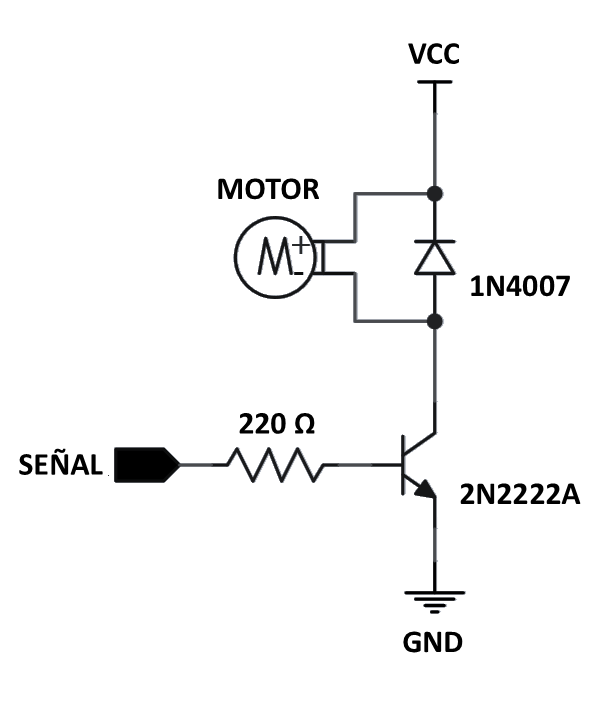
\includegraphics[width=0.5\textwidth,height=\textheight]{Capitulos/../Imagenes/Circuito_motor.png}

}

\caption{\label{fig-circuito_motor}Circuito de control del motor
vibrador}

\end{figure}%

\textbf{Batería}

El uso de baterías de polímero de litio (LiPo) es ampliamente utilizado
en dispositivos portátiles debido a sus características de pequeño
tamaño, bajo peso y facilidad de carga. Para este proyecto, que integra
un microcontrolador XIAO ESP32C3, una pantalla XIAO Round Display, un
sensor GY-906, un sensor MAX30102 y un circuito vibrador, es crucial
seleccionar una capacidad de batería que asegure un funcionamiento
continuo y confiable, considerando el consumo energético de cada
componente involucrado.

El microcontrolador XIAO ESP32C3 presenta un consumo promedio de 74.7 mA
durante su operación activa (Studio 2024), mientras que la pantalla XIAO
Round Display demanda aproximadamente 70 mA (Solution 2024). Por su
parte, el sensor GY-906 tiene un consumo de corriente bajo, en el rango
de 1 a 2 mA (Melexis 2009), el sensor MAX30102 consume entre 0.6 y 1.2
mA durante la medición de la frecuencia cardíaca (Integrated 2015).
Adicionalmente, el motor vibrador registra un consumo estimado de 84 mA
(uElectronics 2024), dependiendo de la intensidad de la vibración y la
carga aplicada.

El consumo total del dispositivo en condiciones de operación máxima
puede alcanzar 232 mA. Sin embargo, este nivel de consumo es poco
probable alcanzarse durante el uso típico del dispositivo,ya que,
durante la mayor parte del tiempo los sensores y la pantalla permanecen
inactivos, y el motor vibrador se enciende únicamente por breves
periodos cada hora. Con el fin de asegurar autonomía del dispositivo y
evitar interrupciones en su funcionamiento, se selecciona una batería de
650 mAh. Este capacidad satisface los requisitos energéticos,
permitiendo el uso prolongado del dispositivo. Además, la batería
seleccionada cumple en tamaño y peso, ajustándose adecuadamente al
diseño del dispositivo.

La Tabla~\ref{tbl-componentes-seleccionados} muestra todos los
componentes seleccionados para el desarrollo del dispositivo.

\begin{longtable}[]{@{}
  >{\raggedright\arraybackslash}p{(\columnwidth - 2\tabcolsep) * \real{0.3182}}
  >{\raggedright\arraybackslash}p{(\columnwidth - 2\tabcolsep) * \real{0.6818}}@{}}
\caption{Tabla de componentes
seleccionados}\label{tbl-componentes-seleccionados}\tabularnewline
\toprule\noalign{}
\begin{minipage}[b]{\linewidth}\raggedright
\textbf{Componente}
\end{minipage} & \begin{minipage}[b]{\linewidth}\raggedright
\textbf{Descripción}
\end{minipage} \\
\midrule\noalign{}
\endfirsthead
\toprule\noalign{}
\begin{minipage}[b]{\linewidth}\raggedright
\textbf{Componente}
\end{minipage} & \begin{minipage}[b]{\linewidth}\raggedright
\textbf{Descripción}
\end{minipage} \\
\midrule\noalign{}
\endhead
\bottomrule\noalign{}
\endlastfoot
XIAO ESP32C3 & Placa de desarrollo compacta con Wi-Fi y BLE \\
XIAO Round Display & Pantalla circular táctil de 1.28 pulgadas \\
GY-906 & Sensor infrarrojo de temperatura sin contacto \\
MAX30102 & Sensor óptico de frecuencia cardíaca \\
Circuito vibrador & Circuito vibrador para notificaciones silenciosas \\
Batería 650 mAh & Batería LiPo recargable \\
\end{longtable}

\begin{enumerate}
\def\labelenumi{\arabic{enumi}.}
\setcounter{enumi}{2}
\tightlist
\item
  \textbf{Diseño del dispositivo}
\end{enumerate}

Una vez seleccionados los componentes principales del dispositivo, el
diseño se centra en crear una carcasa compacta y adecuada en donde los
componentes puedan colocarse sin interferir entre ellos y así mismo el
desarrollo de los circuitos internos de conexión

\textbf{Carcasa:}

La carcasa del dispositivo esta diseñada para ser impresa en 3D y consta
de 3 partes principales y un seguro. La primera parte es la base y esta
es la que está en contacto con la muñeca del usuario, cuenta con ranuras
para el acomodo y fijación de los sensores y que estos queden en
contacto directo con la piel para llevar a cabo las mediciones de forma
adecuada

La parte central de la carcasa es la pieza que va arriba de la base y es
donde se aloja el microcontrolador, el motor vibrador y el interruptor
de encendido. La pieza está diseñada con compartimentos para fijar cada
uno de estos componentes. Por la parte exterior de la carcasa, esta
pieza cuenta con ranuras para colocar las correas que fijan el
dispositivo a la muñeca del usuario.

La parte superior de la carcasa está diseñada con el fin de mantener la
pantalla táctil en su posición y cerrar el dispositivo. Todas las piezas
se ensamblan una con otra por presión, evitando el uso de tornillos.

Adicional, hay una cuarta pieza que es un seguro para fijar el
interruptor de encendido. Esta se coloca por encima del interruptor una
ve esté colocado en su posición en la pieza central. El seguro ensambla
por presión a la pieza y deja fijo el interruptor.

En la figXXX Se observan las tres piezas principales de la carcasa.

\textbf{Diseño de los circuitos}

El diseño de los circuitos se divide en tres circuitos, motor vibratorio
para alarmas circuito Figura~\ref{fig-conexiones} a) , circuito de
sensores y microcontrolador Figura~\ref{fig-conexiones} b), y el
circuito de la batería Figura~\ref{fig-conexiones} c). Cada uno de estos
circuitos está diseñado para mantener las conexiones lo más simples y
cortas posibles. Dado que la placa XIAO ESP32C3 y la pantalla XIAO Round
Display se ensamblan directamente, se omite ese circuito.

\begin{figure}

\centering{

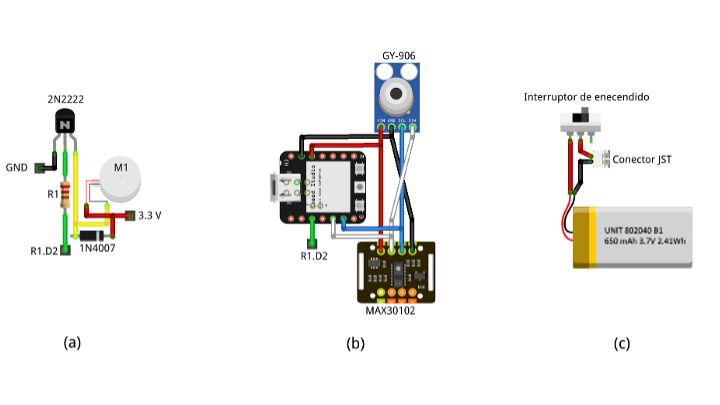
\includegraphics{Capitulos/../Imagenes/Diagrama de conexiones.png}

}

\caption{\label{fig-conexiones}Diagrama de conexiones}

\end{figure}%

El código de colores utilizado en este proyecto, para facilitar las
conexiones, es:

\begin{itemize}
\tightlist
\item
  \textbf{\emph{Rojo:}} Conexión Vcc (3,3 V).
\item
  \textbf{\emph{Negro:}} GND.
\item
  \textbf{\emph{Azul:}} cable de comunicación SCL.
\item
  \textbf{\emph{Blanco:}} cable de comunicación SDA.
\item
  \textbf{\emph{Verde:}} señal de activación del motor.
\item
  \textbf{\emph{Amarillo:}} conexión entre el pin emisor del transistor
  y el motor vibratorio.
\end{itemize}

El Circuito de motor vibrador es un circuito sencillo de control de
motor. Este circuito tiene la finalidad de proteger el microcontrolador
al evitar que el motor se alimente directamente del pin digital del
microcontrolador, si no que lo haga directamente de la alimentación
general del dispositivo, dejando al pin del microcontrolador únicamente
la tarea de dar la señal de activación.

El circuito de los sensores y el microcontrolador tiene la función de
comunicar de forma paralela ambos sensores por protocolo I2C al
microcontrolador.

El circuito de la batería sirve para añadir el interruptor de encendido
y agregar un conector JST que va directo a la pantalla XIAO Round
Display.

En resumen, el diseño del dispositivo está enfocado en optimizar las
conexiones, el espacio y facilitar su montaje, esto a la vez que se
asegura su funcionalidad y ergonomía.

\section{Construcción del
dispositivo}\label{construcciuxf3n-del-dispositivo}

La construcción del dispositivo en tres etapas: La impresión de la
carcasa, la conexión de los componentes electrónicos y la integración y
montaje de todos los elementos.

\textbf{\emph{Carcasa:}} los archivos STL para la impresión de la
carcasa los puedes encontrar en el Anexo XXX

\textbf{\emph{Componentes electrónicos:}} Las conexiones de los
componentes electrónicos se llevan a cabo siguiendo los diagramas de la
imagen XXX. Es importante seguir correctamente los diagramas para
facilitar posteriormente su acomodo dentro de la carcasa.

\textbf{\emph{Integración y montaje:}} Una vez realizadas las
conexiones, se lleva a cabo el montaje de los circuitos dentro de la
carcasa y está se ensambla y se colocan las correas.

En el articulo XXX puede encontrar información más detallada acerca del
diseño y los pasos a seguir para la construcción del dispositivo.

\section{Encuestas e interfaz}\label{encuestas-e-interfaz}

\begin{enumerate}
\def\labelenumi{\arabic{enumi}.}
\tightlist
\item
  Desarrollo del firmware: describe el desarrollo de la interfaz
\item
  Implementación de la encuesta: Explica detalladamente la encuesta y
  porque se eligieron esos preguntas
\end{enumerate}

\section{Calibración}\label{calibraciuxf3n}

\begin{enumerate}
\def\labelenumi{\arabic{enumi}.}
\tightlist
\item
  Calibración de los sensores
\end{enumerate}

\section{Lógica de programación}\label{luxf3gica-de-programaciuxf3n}

XXX Agregar diagrama de flujo del articulo de Francia y después
desglozarlo por partes. XXX

\section{Instrucciones de uso}\label{instrucciones-de-uso}

\begin{enumerate}
\def\labelenumi{\arabic{enumi}.}
\tightlist
\item
  Integración con la plataforma iot
\item
  manejo de los datos
\end{enumerate}

\bookmarksetup{startatroot}

\chapter{Conclusiones}\label{conclusiones}

\section{Discusión}\label{discusiuxf3n}

\subsection{Interpretación de los
resultados}\label{interpretaciuxf3n-de-los-resultados}

\subsection{Contribuciones y
limitaciones}\label{contribuciones-y-limitaciones}

\section{Conclusiones}\label{conclusiones-1}

\bookmarksetup{startatroot}

\chapter*{Referencias}\label{referencias}
\addcontentsline{toc}{chapter}{Referencias}

\markboth{Referencias}{Referencias}

\phantomsection\label{refs}
\begin{CSLReferences}{1}{0}
\bibitem[\citeproctext]{ref-Calixto2021}
Aguirre, Verónica Ivette Calixto. 2021. {«Thermal comfort studies»}.
Universidad Nacional Autonoma de México.
\url{http://132.248.9.195/ptd2021/septiembre/0814603/Index.html}.

\bibitem[\citeproctext]{ref-ASHRAE55}
American Society of Heating, Refrigerating and Air-Conditioning
Engineers, Inc. 2017. \emph{Thermal Environmental Conditions for Human
Occupancy}. ASHRAE Standard 55-2017. American Society of Heating,
Refrigerating; Air-Conditioning Engineers, Inc.

\bibitem[\citeproctext]{ref-Bogatu2023}
Bogatu, Dragos Ioan, Jun Shinoda, José Joaquín Aguilera, Bjarne W.
Olesen, Futa Watanabe, Yosuke Kaneko, y Ongun B. Kazanci. 2023. {«Human
physiology for personal thermal comfort-based HVAC control -- A
review»}. \emph{Building and Environment} 240 (julio): 110418.
\url{https://doi.org/10.1016/J.BUILDENV.2023.110418}.

\bibitem[\citeproctext]{ref-CHEUNG2019}
Cheung, Toby, Stefano Schiavon, Thomas Parkinson, Peixian Li, y Gail
Brager. 2019. {«Analysis of the accuracy on PMV -- PPD model using the
ASHRAE Global Thermal Comfort Database II»}. \emph{Building and
Environment} 153: 205-17.
https://doi.org/\url{https://doi.org/10.1016/j.buildenv.2019.01.055}.

\bibitem[\citeproctext]{ref-Enescu2017}
Enescu, Diana. 2017. {«A review of thermal comfort models and indicators
for indoor environments»}. \emph{Renewable and Sustainable Energy
Reviews} 79 (noviembre): 1353-79.
\url{https://doi.org/10.1016/J.RSER.2017.05.175}.

\bibitem[\citeproctext]{ref-Fanger1970}
Fanger, P. O. 1970. \emph{Thermal Comfort: Analysis and Applications in
Environmental Engineering}. Copenhagen: Danish Technical Press.
\url{https://archive.org/details/thermalcomfortan0000fang}.

\bibitem[\citeproctext]{ref-infonavit2024regiones}
Infonavit. 2024. {«Listado de Regiones Bioclimáticas»}.
\url{https://portalmx.infonavit.org.mx/wps/wcm/connect/005dcf74-d918-41aa-acfa-927e7b33d98a/12.\%2BAnexo\%252B1.\%252BListado\%252Bde\%252Bregiones\%252Bbioclim\%25C3\%25A1ticas.pdf?MOD=AJPERES&CONVERT_TO=url&CACHEID=ROOTWORKSPACE-005dcf74-d918-41aa-acfa-927e7b33d98a-mmCFC0}.

\bibitem[\citeproctext]{ref-max30102_datasheet}
Integrated, Maxim. 2015. \emph{MAX30102 High-Sensitivity Pulse Oximeter
and Heart-Rate Sensor for Wearable Health}.
\url{https://www.alldatasheet.com/datasheet-pdf/view/859400/MAXIM/MAX30102.html}.

\bibitem[\citeproctext]{ref-Judson2022}
Judson, Emily, Oscar Fitch-Roy, y Iain Soutar. 2022. {«Energy democracy:
A digital future?»} \emph{Energy Research and Social Science} 91
(septiembre). \url{https://doi.org/10.1016/j.erss.2022.102732}.

\bibitem[\citeproctext]{ref-Chatellier2020}
Lorentzen, Diego M. P. Chatellier, y Michael A. McNeil. 2020.
{«Electricity demand of non-residential buildings in Mexico»}.
\emph{Sustainable Cities and Society} 59 (agosto).
\url{https://doi.org/10.1016/j.scs.2020.102165}.

\bibitem[\citeproctext]{ref-mlx90614_datasheet}
Melexis. 2009. \emph{MLX90614 Infra Red Thermometer in TO-39}.
\url{https://www.melexis.com/en/documents/documentation/datasheets/mlx90614-datasheet}.

\bibitem[\citeproctext]{ref-IPCC2022}
Mitigation of Climate Change, Climate Change 2022 -. 2022. {«Mitigation
of Climate Change Climate Change 2022 Working Group III contribution to
the Sixth Assessment Report of the Intergovernmental Panel on Climate
Change»}.
\url{https://www.ipcc.ch/site/assets/uploads/2018/05/uncertainty-guidance-note.pdf.}

\bibitem[\citeproctext]{ref-Olabi2023}
Olabi, A. G., Mohammad Ali Abdelkarem, y Hussam Jouhara. 2023. {«Energy
digitalization: Main categories, applications, merits, and barriers»}.
\emph{Energy}. Elsevier Ltd.
\url{https://doi.org/10.1016/j.energy.2023.126899}.

\bibitem[\citeproctext]{ref-olgyay1963}
Olgyay, V., D. Lyndon, J. Reynolds, y K. Yeang. 1963. \emph{Design with
Climate: Bioclimatic Approach to Architectural Regionalism - New and
expanded Edition}. Princeton University Press.
\url{https://books.google.com.mx/books?id=RRQ-CgAAQBAJ}.

\bibitem[\citeproctext]{ref-Ods2015}
Organización de las Naciones Unidas. 2015. {«Transforming our world: the
2030 Agenda for Sustainable Development»}.
\url{https://digitallibrary.un.org/record/3923923}.

\bibitem[\citeproctext]{ref-owid-ghg-emissions-by-sector}
Ritchie, Hannah. 2020. {«Sector by sector: where do global greenhouse
gas emissions come from?»} \emph{Our World in Data}.

\bibitem[\citeproctext]{ref-BNE2022}
Secretaría de Energía. 2023. {«Balance Nacional de Energía Preliminar
2022»}.
\url{https://www.gob.mx/cms/uploads/attachment/file/841526/BNE_2022.pdf}.

\bibitem[\citeproctext]{ref-xiaodisplay}
Solution, ETA. 2024. \emph{ETA6003 2.5A, 3MHz Switching Charger with
Dynamic Power Path Management}. ETA Solution.
\url{https://files.seeedstudio.com/wiki/round_display_for_xiao/charge-IC-datasheet.pdf}.

\bibitem[\citeproctext]{ref-xiaoesp32c3}
Studio, Seeed. 2024. {«Seeed Studio XIAO ESP32C3 Development Board»}.
\url{https://www.seeedstudio.com/Seeed-XIAO-ESP32C3-p-5431.html?srsltid=AfmBOopHrrta3vMhxj9CZJasHKtro5S9tVjwzPT3-KtKiNUV8CeFVebb}.

\bibitem[\citeproctext]{ref-IPCC2023}
Synthesis Report, Climate Change 2023: 2023. {«IPCC, 2023: Climate
Change 2023: Synthesis Report. Contribution of Working Groups I, II and
III to the Sixth Assessment Report of the Intergovernmental Panel on
Climate Change {[}Core Writing Team, H. Lee and J. Romero (eds.){]}.
IPCC, Geneva, Switzerland.»} Editado por Paola Arias, Mercedes
Bustamante, Ismail Elgizouli, Gregory Flato, Mark Howden, Carlos
Méndez-Vallejo, Joy Jacqueline Pereira, et~al. Intergovernmental Panel
on Climate Change.
\url{https://doi.org/10.59327/IPCC/AR6-9789291691647}.

\bibitem[\citeproctext]{ref-uelectronics_vibration_motor}
uElectronics. 2024. {«Motor de Vibración 5V»}.
\url{https://uelectronics.com/producto/motor-vibracion-5v/?srsltid=AfmBOoobMBx68FsKl3OQeHRxlqV72c0WFDIICCubVzyQFrHrNYflB-w4}.

\end{CSLReferences}




\end{document}
